\chapter{Why All Writing Sounds the Same Now}

This lecture is not mathematical in the literal sense. There is no blackboard, no symbolic derivation, and no visible equation to recover from the video. But there is a real formal spine. Macfarlane treats writing as a problem of relation: relation between subject and sentence, between perception and language, between river flow and prose flow, between notebook fragment and finished book, between rational explanation and wonder. The lecture begins with biography, moves into sentence mechanics, widens into process and worldview, and closes with revision, precision, and resistance to standardized prose. We will keep that order, because the argument accumulates.

\begin{remark}
The formulas in this chapter are schematic compressions of distinctions the lecture makes explicitly in speech. They are not recovered lecture notation. Their purpose is to make the structure of the argument easier to see.
\end{remark}

\section{Mountains, Light, and the Failure of Capture}

The lecture opens from admiration and biography. The first question is not ``What is your theory of writing?'' but rather: where does this sensitivity come from? Macfarlane's answer is bodily before it is literary. Mountains sharpen sensation, demand alertness, and wear away the ordinary shell of the self. Danger does not merely threaten; it trains attention.

In the lecture's own sequence, the causal chain is almost immediate:
\begin{equation}
\text{danger} \longrightarrow \text{alertness} \longrightarrow \text{openness} \longrightarrow \text{heightened attention}.
\end{equation}
What matters here is that sensibility is not treated as temperament alone. It is cultivated in intense places: brighter light, sharper snow, air felt like wire in the nose, and the constant need to assess risk. The mountain is therefore not only scenery. It is a school of perception.

That biographical opening leads directly to light. The host gives a failed sunset anecdote: a blood-orange sky seen from an airplane, a phone left unused, and then grief at not having words adequate to the sight. This is the lecture's first real craft problem. How do we write what plainly outruns language?

Macfarlane's answer is a refusal. One should abandon what he calls the dream of correspondence. In schematic form:
\begin{align}
\text{correspondence} &\not\Rightarrow \text{adequate writing of light},\\
\text{artifice} &\Rightarrow \text{evocation of perception}.
\end{align}
Light moves too quickly, shifts too rapidly, and changes texture too constantly for language ever to meet it point for point. If we cling to one-to-one matching, we remain stuck in the feeling of failure. The lecture insists that the better move is not despair but method: once we stop demanding exact capture, we can lean into metaphor, distortion, and formal construction.

\begin{definition}
By \emph{representation of perception} the lecture means not the thing in itself, but the thing as encountered through a particular body, mind, mood, motion, and field of attention.
\end{definition}

This is why the host's analogy to impressionism matters. The aim is not possession. Macfarlane explicitly resists the verb ``capture,'' because captured nature ceases to be free and becomes a captive object. The better analogy is impressionist painting: not a sealed transfer of the world, but a shaped registration of how the world arrived to perception.

\section{Water, Punctuation, and the Small Mechanics of Thought}

From light the lecture moves naturally to water. The shift is important: once correspondence has been rejected, we need a constructive principle. Water provides it. Macfarlane says there is no single grammar of water. That is the chapter's next formal claim, and it blocks a very common simplification:
\begin{equation}
\text{river language} \neq \text{fast language only}.
\end{equation}

The host helps here by naming different river forms. Rivers can pool, pause, meander, run straight, or break into rapids. So can prose. The lesson is not merely that writing should ``flow,'' but that different forms of water call for different formal responses. A lake passage and a rapid passage should not sound the same.

We can state the taxonomy exactly as the lecture implies it:
\begin{itemize}
\item still or pooled water asks for slower rhythm and wider spacing,
\item meandering water allows drift, turn, and delayed arrival,
\item straight water may permit direct propulsion,
\item rapid water invites broken urgency, accumulation, and pressure.
\end{itemize}

Once that has been said, the lecture narrows from large forms to tiny operators. Macfarlane is, by his own description, obsessed with punctuation and prepositions. The dash comes first. A full stop closes. The dash remains fluid. Meaning can move backward through it and forward through it. The lecture's point is not merely stylistic preference. Punctuation is treated as traffic control for meaning.

The lecture then turns to the prepositional ladder. This is one of its clearest formal structures:
\begin{equation}
\text{about river} \longrightarrow \text{with river} \longrightarrow \text{by river}.
\end{equation}
To write \emph{about} a river is to describe it as object. To write \emph{with} a river is already to shift agency, so that writer and river become co-thinking presences. To be written \emph{by} river is a much stronger claim: the writer becomes conduit or channel. The lecture explicitly marks this as a metaphysical distance, not a grammatical quibble.

The host's paraphrase is exact and helpful: almost as if the river becomes co-author. That restatement should be preserved, because it makes the abstract point plain without weakening it.

From punctuation and prepositions, the lecture widens into rhythm. Poetry trains us to hear rhythm, but nonfiction also works on what Macfarlane calls the reader's ``mind's ear.'' It does not operate only by propositions, facts, or arguments. It also acts through cadence, pattern, rhyme, and internal echo. In that sense the lecture gives us a simple first-line schema:
\begin{equation}
\text{first line} = \text{sound pattern} + \text{puzzle} + \text{conceptual opening}.
\end{equation}

This is why ``The wind was rising, so I went to the wood'' is such a strong example. It gives alliteration in \emph{wind} and \emph{wood}; it gives rhythm; and it gives a puzzle. Why go into the wood when the wind is rising? By contrast, ``12{,}000 years ago, a river is born'' is less rhythmic but more ominous. Something happened far back in time; a puzzle opens at once. The lecture's real lesson is that first lines can be tuned differently, but they must do work immediately.

\section{Writing Speed as a Formal Problem}

\subsection{Question \& Answer}

\paragraph{Question.} How do we write speed?

\paragraph{Answer.} Not by reducing the matter to ``short sentences'' or ``fast sentences.'' The lecture's answer is more exact: we create a syntax that tumbles, contracts, and refuses hierarchy.

Macfarlane gives a concrete example from his river writing, and the lecture makes the example visibly central by placing the prose itself on screen. This is the one frame in the lecture that must remain in the notes as direct visual evidence of the pedagogical move.

\begin{figure}[ht]
\centering

\includegraphics[width=0.92\textwidth]{lecture_17_figure_02.png}
\caption{On-screen river passage illustrating a syntax of speed and panic}
\end{figure}

The image matters because the lecture is not merely talking \emph{about} vivid prose. It pauses to inspect the prose itself. The displayed passage is dense, accumulative, and breathless. Even the screen layout helps: the eye meets a long block rather than a neatly segmented set of short units.

Macfarlane then explains the mechanism. In compact form:
\begin{equation}
\#(\text{and}) \uparrow,\qquad \ell_{\text{clause}} \downarrow,\qquad a_{\text{verb}} \uparrow
\Longrightarrow \text{panic and speed} \uparrow.
\end{equation}
Here \(\ell_{\text{clause}}\) is the average clause length, and \(a_{\text{verb}}\) names the pressure exerted by active verbs.

The lecture also gives a local equivalence:
\begin{equation}
\text{``and''} \sim \text{dash}.
\end{equation}
That is, the repeated conjunction plays the role that the dash played earlier. It keeps the sentence running. It prevents full hierarchical sorting. It refuses the calm achieved by full stops and well-tiered subordination.

We can reconstruct the derivation step by step:
\begin{enumerate}
\item Begin not with a clean sentence but with prose already in motion.
\item Repeat ``and'' so that the syntax keeps tumbling forward.
\item Let the clauses between the conjunctions shorten as pressure rises.
\item Push agency into bodily verbs: slammed, exploded, punching, ramming, grabbing, hauling.
\item Drop the article in ``river,'' so that the force feels less like an object and more like an active medium.
\item Result: the reader becomes breathless, because the prose withholds the ordinary places where breathing would be reset.
\end{enumerate}

The dropped article is especially revealing. ``The river'' remains nameable object. ``River'' becomes force. The lecture lingers on this small choice because it shows how microscopic grammar changes the ontology of the scene.

\begin{figure}[ht]
\centering
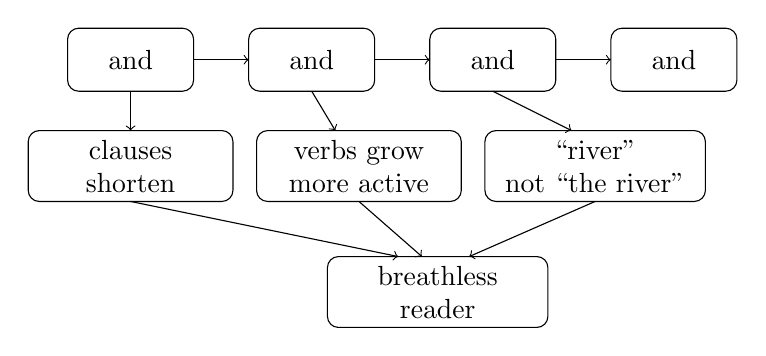
\begin{tikzpicture}[x=1cm,y=1cm]
\draw[rounded corners] (-5.3,1.2) rectangle (-3.7,2.0);
\node at (-4.5,1.6) {and};
\draw[rounded corners] (-3.0,1.2) rectangle (-1.4,2.0);
\node at (-2.2,1.6) {and};
\draw[rounded corners] (-0.7,1.2) rectangle (0.9,2.0);
\node at (0.1,1.6) {and};
\draw[rounded corners] (1.6,1.2) rectangle (3.2,2.0);
\node at (2.4,1.6) {and};

\draw[->] (-3.7,1.6) -- (-3.0,1.6);
\draw[->] (-1.4,1.6) -- (-0.7,1.6);
\draw[->] (0.9,1.6) -- (1.6,1.6);

\draw[rounded corners] (-5.8,-0.2) rectangle (-3.2,0.7);
\node[align=center] at (-4.5,0.25) {clauses\\shorten};

\draw[rounded corners] (-2.9,-0.2) rectangle (-0.3,0.7);
\node[align=center] at (-1.6,0.25) {verbs grow\\more active};

\draw[rounded corners] (0.0,-0.2) rectangle (2.8,0.7);
\node[align=center] at (1.4,0.25) {``river''\\not ``the river''};

\draw[rounded corners] (-2.0,-1.8) rectangle (0.8,-0.9);
\node[align=center] at (-0.6,-1.35) {breathless\\reader};

\draw[->] (-4.5,1.2) -- (-4.5,0.7);
\draw[->] (-2.2,1.2) -- (-1.9,0.7);
\draw[->] (0.1,1.2) -- (1.1,0.7);

\draw[->] (-4.5,-0.2) -- (-1.1,-0.9);
\draw[->] (-1.6,-0.2) -- (-0.8,-0.9);
\draw[->] (1.4,-0.2) -- (-0.2,-0.9);
\end{tikzpicture}
\caption{Analytical reconstruction of the sentence mechanics in the river passage}
\end{figure}

This is the lecture's clearest worked formal example. The payoff is not abstract. Macfarlane says that when we read such a passage, we ourselves do not know when to breathe. The sentence reproduces, not the event itself, but a bodily analog of being buried in a rapid.

\section{From Notebook to Book}

\subsection{Question \& Answer}

\paragraph{Question.} How do notes become books?

\paragraph{Answer.} Not by direct expansion of a miniature book already present in the notebook. The notebook is not a reduced chapter. It is an encrypted trigger system.

The lecture slows down sharply here, and that slowdown should be preserved. After the intensity of the speed example, Macfarlane moves into stages. His books take years. They involve repeated journeys, meetings with people, and prolonged fieldwork. He prefers small notebooks, roughly A6, not because they are elegant, but because they bend, fit in a pocket, and can be used in real conditions.

Into these notebooks go what he calls \emph{qualia}: fragments of subjective perception. Images. shards of dialogue. bits and bobs. What is important is that the notes are not continuous. They are discontinuous, messy, and intensely private. The lecture emphasizes this repeatedly. No one else could follow them linearly.

The process can be written schematically as
\begin{equation}
\text{fragment} \longrightarrow \text{mnemonic trigger} \longrightarrow \text{memory expansion} \longrightarrow \text{pattern recognition} \longrightarrow \text{heart work}.
\end{equation}

The host contributes a valuable metaphor here. A small page or card becomes a condensation surface. Thought has been present like vapor, but the page causes it to gather. Macfarlane agrees and sharpens the point: paper and pen do things that keyboard and pixel do not. The note is ``fresh from the fire,'' still hot, not yet communicable.

The next stage comes at home, when the notebooks are reread on screen. Each fragment becomes the visible end of a thread. We pull the thread, and the larger scene opens around it again. That is the lecture's most precise description of the memory process. The note is not the memory. It is the handle by which memory can be recovered.

One can summarize the pipeline even more compactly:
\begin{equation}
\text{notebook work} \longrightarrow \text{heart work}.
\end{equation}
Macfarlane invokes Rilke in paraphrase here, and the exact wording is uncertain in the transcript. But the distinction is clear enough. Immediate noticing is not yet the book. The book begins when noticed images are returned to, related, and understood in their resonance with other images.

That is where pattern recognition enters. Macfarlane's example from \emph{Underland} is the open hand. He notices the hand first in cave stencil art, where the hand is not printed positively but leaves behind its own absence. He then sees versions of that shape again in later journeys, including modern graffiti and the open hand of greeting and welcome. What begins as repeated image becomes motif.

The lecture's motif model can be stated as
\begin{equation}
\text{repeated image} \longrightarrow \text{recurrence across journeys} \longrightarrow \text{pattern lighting up}.
\end{equation}

The phrase ``lighting up'' is important. A motif does not merely recur; it becomes active for writer and reader. At that point the book is no longer a heap of notes. It is becoming an organized field of echoes.

\section{Wonder, Scale, and Unlearning}

\subsection{Question \& Answer}

\paragraph{Question.} What does it mean to unlearn?

\paragraph{Answer.} The lecture answers this by placing child-perception, wonder, scale, and the river's agency into one sequence. Unlearning is not ignorance. It is the difficult undoing of a narrowed adult frame.

The immediate trigger is Macfarlane's anecdote about his son. He says he is writing a book called \emph{Is a River Alive?}; the child replies, in effect, ``Of course.'' The host sees at once what is at stake. Children sometimes hold a more enchanted, less over-rationalized picture of the world. Macfarlane pushes the point further by calling wonder an essential survival skill.

The rainbow example then performs two tasks at once. First, it defines wonder as jaw-dropped astonishment. Second, it refuses the lazy opposition between science and wonder. A rainbow can be explained as prismatic separation of wavelengths by water, and yet the explanation does not exhaust the phenomenon. In fact, the lecture suggests that explanation may intensify wonder when it is held properly.

Scale becomes the next operator. Blake's grain of sand is tiny and yet opens toward infinity. Macfarlane then generalizes:
\begin{equation}
\text{micro scale} < \text{human scale} < \text{macro scale}.
\end{equation}
The symbols should not be taken too literally. The lecture's point is not numerical order but nested juxtaposition. We ordinarily inhabit the human scale, but good writing can place that scale beside microscopic and cosmic orders without flattening them into one viewpoint.

This is why the lecture invokes the microscope and telescope in the early modern period. Galileo sees mountains on the moon; van Leeuwenhoek peers into a droplet and finds life teeming there. Technology breaks open scale. Writing, for Macfarlane, can do something analogous by nesting scales within one another.

Then comes the hard philosophical turn. The host names the ``blinders of rationality.'' Macfarlane agrees. To believe that a river is alive in a way that exceeds the mere sum of the organisms in it requires unlearning. Rationalism, in the lecture's metaphor, is not a total floodlight but a moving lamp in a cave. It lights a patch. Much remains beyond the beam.

The river journey supplies the lived version of this claim. The discharge figure is one of the few places where the lecture briefly becomes numerically explicit:
\begin{align}
Q_{\text{normal}} &\approx 150\,\mathrm{m^3\,s^{-1}},\\
Q_{\text{observed}} &\approx 275\,\mathrm{m^3\,s^{-1}},\\
\frac{Q_{\text{observed}}}{Q_{\text{normal}}} &\approx 1.83.
\end{align}
So the river was running at nearly double its ordinary flow. The calculation is simple, but it matters. The physical excess is part of the argument. This was not reflective musing beside gentle water. It was prolonged bodily abrasion: swimming, tumbling, striking rocks, living under the force of a high river.

The lecture's deeper claim is that the river did the unlearning. It did so physically and metaphysically. It ceased to appear as dead matter and began to appear as force, will, presence, and agency. Macfarlane describes a river-being, even a godlike presence, and is careful not to claim perfect representation of it. Once again, the lesson is earlier than the content:
\begin{equation}
\text{extreme encounter} \longrightarrow \text{unlearning} \longrightarrow \text{analogical registration, not full capture}.
\end{equation}

The chapter should preserve the caution here. The lecture does not ask us to endorse a doctrine. It asks us to see how language changes once the writer has been pressed beyond a merely objectifying relation to the world.

\section{Questions as Portals, and Other People as Co-Writers}

\subsection{Question \& Answer}

\paragraph{Question.} How can a simple question open into a whole book?

\paragraph{Answer.} Because the right question is not a conclusion waiting for a slogan. It is a portal.

The host notices that Macfarlane's books often begin with narrow questions: Why climb mountains? Can a forest think? Does a mountain remember? Is a river alive? Macfarlane agrees and immediately offers a cautionary example. George Mallory's famous ``Because it's there'' does not help much. It has become legendary, but it closes the inquiry just where a book needs it to open.

That gives us the lecture's next strong formal model:
\begin{equation}
\text{simple question} \longrightarrow \text{narrow portal} \longrightarrow \text{large chamber of complexity}.
\end{equation}
The caving metaphor is precise. A seemingly modest opening leads, after difficulty, to a huge subterranean chamber. The host's Narnia analogy helps. The wardrobe is ordinary at the threshold; it becomes expansive only after passage through it.

Macfarlane then describes two practical planning devices. The first is to find the portal question. The second is to write a letter to the future self at the start of the book. Because the books take years, the writer and the world both change. The letter is therefore not law. It is an early map of hope: what the book may become, what metaphors may organize it, what work it may do in the world.

The lecture also adds a third tool: pinned quotations. For \emph{Is a River Alive?} Macfarlane singles out Ursula Le Guin's phrase about ``a great reach outward of mind and imagination.'' That phrase becomes a discipline of thought. To answer the river question as an adult formed by rationalism requires precisely such a reach outward.

At this point the host asks how much book-writing is plan and how much adventure. Macfarlane answers with another river analogy, and this one is excellent. Writing the book felt less like drifting downstream than like walking upstream in a river. When both feet are planted, one is stable. The moment of danger and progress comes when a foot is lifted for the next step. In the lecture's logic:
\begin{equation}
\text{rest} = \text{relative stability},\qquad
\text{next step} = \text{unbalance} + \text{progress}.
\end{equation}
This is a formal statement of a practical truth. The book is most unstable not when we stop, but when we move.

The section then widens to other people. Macfarlane resists the idea that nature writing is properly people-less. He wants the book populated by voices, specialists, companions, and interlocutors. The right people are not distractions from the landscape; they are additional forms of intelligence within it. That is why he can speak of travel companions almost as co-writers.

The host's metaphor of conversation as fire-building is worth keeping. A real conversation is not two intersecting monologues. It is co-creation. Neither person could have made the same thing alone. The lecture explicitly imports this into writing.

The same enlargement happens across forms. Poetry, libretti, and songwriting teach Macfarlane things prose alone may conceal: singability, sound currents, transitions between words, looseness of image, and the productive value of friction. His discussion of songwriting is especially useful. In song, elements can sit slightly off beat, slightly in friction, and the mismatch becomes feature rather than bug. He calls this glitch. What looks like error may be exactly the formal cue that gives the piece its strangeness.

That lesson carries back into prose. If one wants to register uncanny experience, fully smoothed syntax may be the wrong instrument.

\section{Precision, Revision, and Distinctiveness}

The lecture's final movement is rapid but coherent. It gathers words, place-names, language death, revision, work discipline, automation, astonishment, and the reader's bodily participation. The best way to hold it together is to see that each topic answers the title's complaint about sameness.

Macfarlane begins with words. He likes glossaries not as displays of erudition, but as instruments of precision. He insists that precision is not the enemy of lyricism. On the contrary, precision may be one of lyricism's conditions. Old English kennings such as ``bone-cage'' and ``whale-road'' show language's power to fuse image and naming. Seamus Heaney's phrase ``the palp and heft of language'' points in the same direction: words can be weighed, handled, felt.

The lecture then turns to Scottish Gaelic and related naming traditions. Some transcript spellings in this stretch are uncertain, and one should verify the exact orthography later. But the structural point is clear. A single local word may compress an entire paragraph of description. Many place-names function as a kind of geographic intelligence. They do not merely label mountains; they encode shape, orientation, or relation to the surrounding land. The lecture jokingly calls this a ``Gaelic positioning system.''

The same section defines language death with great clarity. A language dies when its last living speaker dies and it is no longer being transmitted. Recordings may survive, but lived passage does not. The lecture then makes the stronger claim:
\begin{equation}
\text{language death} \longrightarrow \text{loss of knowledge}.
\end{equation}
Indeed, some knowledge is not cleanly alienable from the language that bears it. So language death is not only lexical loss; it is biocultural collapse.

Revision comes next. Macfarlane describes himself as a messy writer and gives two analytic models. The first is the potter model:
\begin{align}
\text{wet mass of clay} &\longrightarrow \text{spin} \longrightarrow \text{shape} \longrightarrow \text{ornament},\\
\text{raw draft} &\longrightarrow \text{repeated passes} \longrightarrow \text{form} \longrightarrow \text{finish}.
\end{align}
The analogy is good because it rejects the fantasy of immaculate first composition. Form emerges through labor on something initially muddy.

The second is the mosaic model:
\begin{equation}
\text{set piece}_1 + \text{set piece}_2 + \cdots + \text{set piece}_n
\longrightarrow \text{chapter by assembly}.
\end{equation}
Macfarlane does not require linear drafting. If one part of the book is blocked, another part can be written first. This is practical advice, not merely autobiography.

The lecture adds two work habits here. First, when one stops for the day, leave the next sentence known. Second, if stuck, jump downstream and write another part. Both strategies are ways of preserving momentum. They also return us to the lecture's recurrent refrain: ass on chair. Show up. Even a paragraph is a paragraph more than the book had the day before.

Then comes automation. Macfarlane is clear that smoothing tools improve average prose while harming distinctive prose. His example is telling: verbless paragraphs, clipped fragments, paragraph breaks used as rhythmic pressure, and syntactic deviations that grammar checkers dislike precisely because they are deliberate. In formal shorthand:
\begin{align}
\text{tool smoothing} \uparrow &\Longrightarrow \text{average competence} \uparrow,\\
\text{tool smoothing} \uparrow &\Longrightarrow \text{distinctiveness} \downarrow.
\end{align}
This is one of the lecture's cleanest late claims, and it belongs at the heart of the title question. Writing sounds the same when it is forced toward average repair.

There is one more power the lecture wants to preserve: visceral transmission. In discussing claustrophobic passages from \emph{Underland}, Macfarlane argues that prose can act not only on the reader's mind but on the body. Readers stop reading because the passage makes them clench, speed up, or seek open air. William Golding's phrase ``sympathetic kinesthesia'' is useful here. A sentence can provoke bodily response. That is not the opposite of craft. It is one of craft's highest achievements.

Late in the lecture, the host raises the old advice to remove needless words. Macfarlane's answer is judicious. Sometimes subtraction is right. Walter Pater's ``hard, gem-like flame'' stands behind that tradition. Sometimes, however, addition is right. Each landscape and each encounter asks for a bespoke presence of language. The important point is not a universal doctrine of reduction, but judgment.

The same is true of astonishment. Hyperbole is dangerous. Purple prose lies. The lecture insists that astonishment is best preserved not by overstatement but by exactness, restraint, and the refusal to over-explain. When everything is fully dotted and crossed, the reader has nowhere to enter. Good writing leaves space for co-creation.

That is why the lecture ends so well on the sentence from \emph{Is a River Alive?}: in English there is no verb ``to river,'' but what could be more of a verb than a river? The sentence is at once finished thought and send-off. It reopens the portal at the level of a single line. We assent to it, then think again, and then the conceptual chamber opens behind it.

\section{Summary}

The lecture begins with mountains and ends with distinctiveness, but the line between them is continuous. Intense places train attention; failed correspondence forces a turn toward artifice; water teaches that form must vary with subject; punctuation and prepositions act as real operators; speed is written through coordination, contraction, and verb pressure; notebooks become books only through memory, recurrence, and heart work; wonder depends on our ability to place scales beside one another and to unlearn a narrow rationalism; books are organized by portal questions; and late craft consists in preserving precision, bodily force, and individuality against flattening.

If we compress the whole lecture into one final relation, it is this:
\begin{equation}
\text{attention} + \text{form} + \text{judgment} \Longrightarrow \text{writing with a distinct mind and ear}.
\end{equation}
That is the lecture's answer to sameness. Writing sounds the same when it loses its ear, its risk, and its exact relation to the thing encountered. It becomes alive again when the sentence is made answerable to perception, pressure, mystery, and voice.